\section{Semaforo disabilitabile}

Per la realizzazione del semaforo completo si è proceduto ad implementare un ulteriore ingresso (En). Tale ingresso svolge la funzione di abilitare il semaforo: in modalità abilitato il circuito realizzato si deve comportare come descritto precedentemente, mentre qualora si abbia il semaforo disabilitato devono alternarsi ciclicamente gli stati:
\begin{center}
tutti i LED spenti $\longleftrightarrow$ LED giallo acceso
\end{center}
Essendo arbitraria la codifica del valore di abilitazione è stato imposto che il semaforo sia abilitato
per $En = 1$, trovando più semplice implementare in tal modo la logica necessaria; si è inoltre optato per una FSM di Mealy in modo da non dover introdurre altri D-Latch.

Ad $En = 1$ gli output del circuito e le transizioni tra gli stati corrispondono a quelli del circuito senza Enable realizzato precedentemente, mentre ad $En = 0$ il circuito compie un ciclo di due soli stati, ed ha dunque transizioni diverse; uno schema della FSM ideata è mostrato in \fig{enstates}.

\begin{figure}[h]
	\centering
	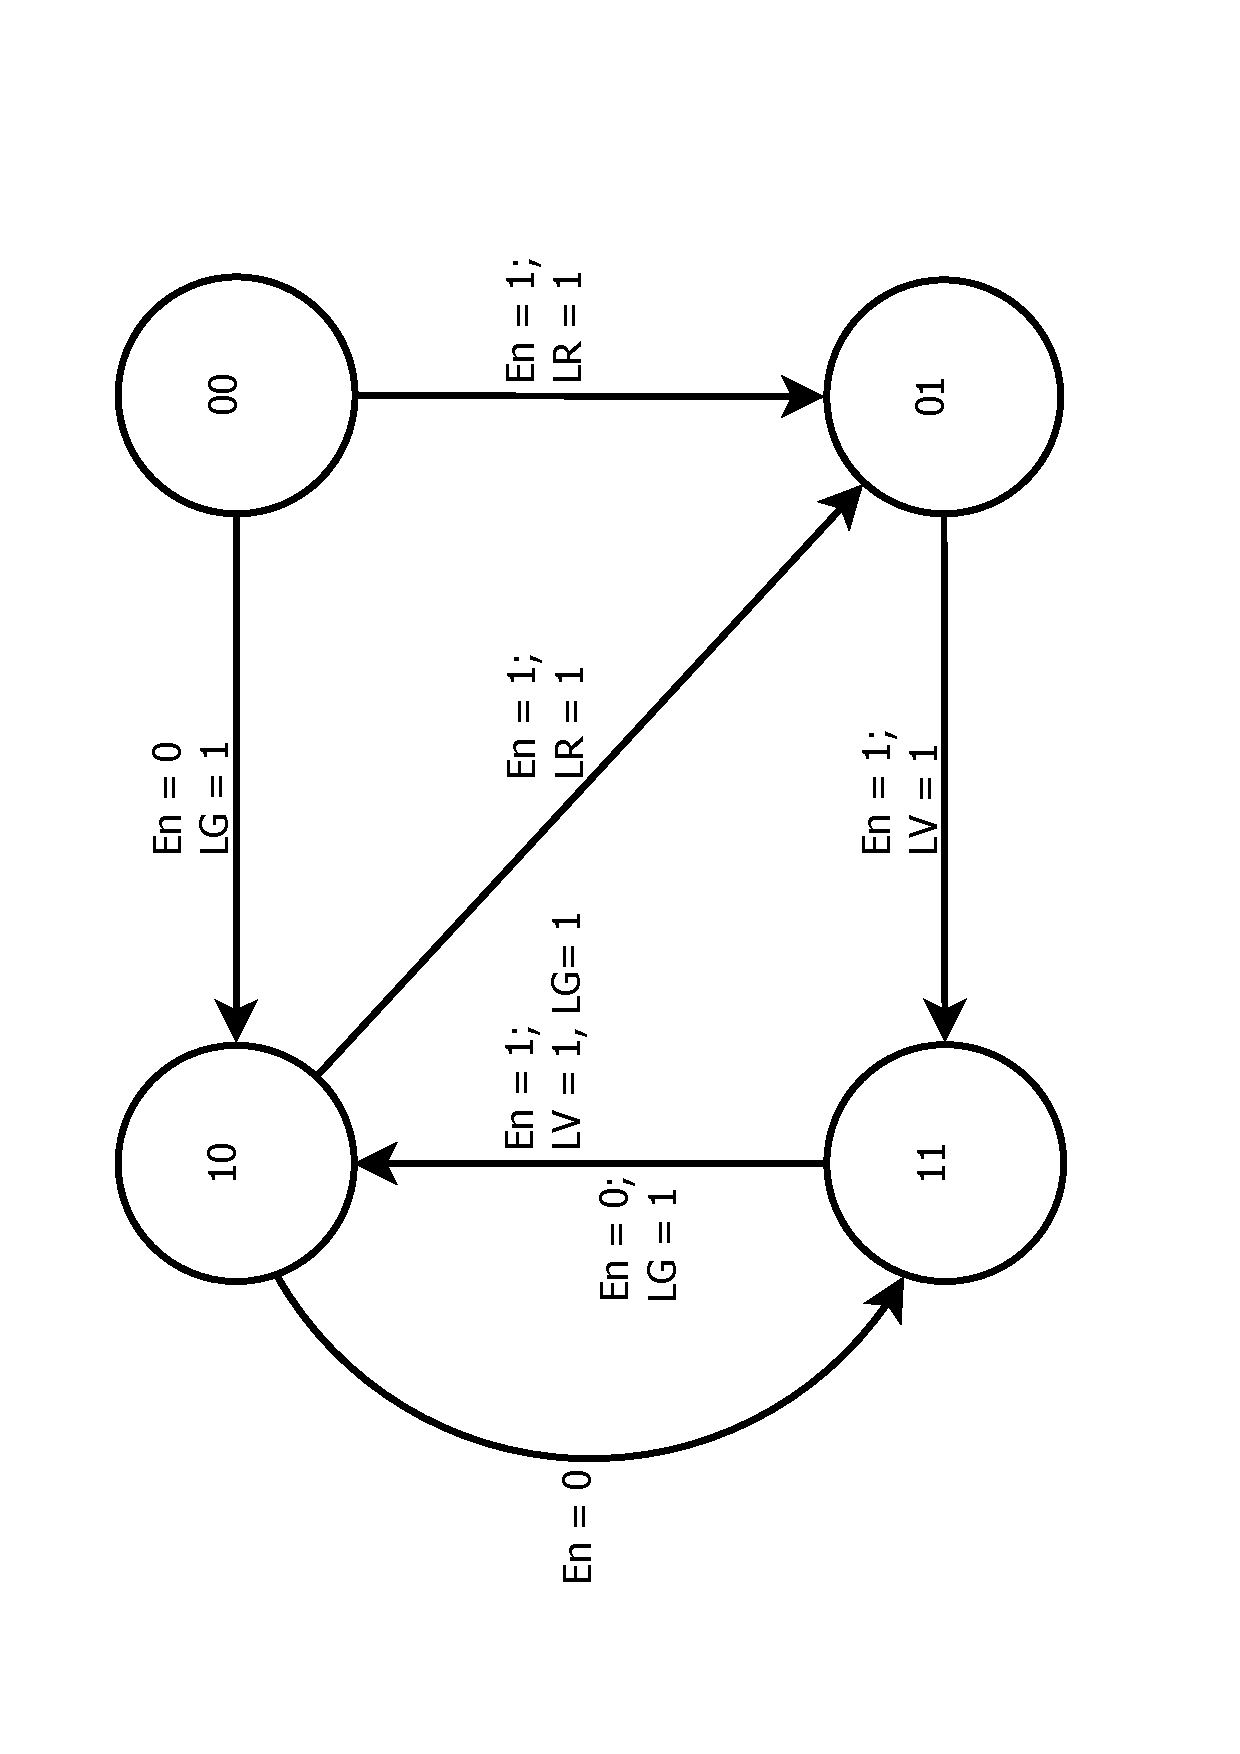
\includegraphics[scale=0.4,angle=-90,origin=c,trim={1.5cm 2.5cm 2.5cm 3cm},clip]{stati_con_enable.pdf}
	\caption{Stati della FSM di Mealy; gli output non indicati sono a 0.}
	\label{fig:enstates}
\end{figure}

Una logica che realizzi quanto desiderato è:
$$b_0^{n+1} =  \overline{b_{1}^{n} \cdot b_{0}^{n}} \qquad b_1^{n+1} = b_0^{n} + \overline{En}$$
$$LV = b_1 \cdot En \qquad LG = \overline{b_0} \qquad LR = \overline{b_1}$$
Si riporta la tabella di verità in \tab{tran2}; si tenga presente che alcune delle transizioni determinate da una variazione di $En$ non sono sincrone (nello specifico, gli stati che non fanno parte del ciclo ``percorso'' a semaforo disattivato (Enable 0) passano a stati del ciclo non appena $En$ passa da 1 a 0) e che inoltre, essendo la nostra una macchina di Mealy, gli output possono variare (in modo asincrono) non appena varia $En$, anche se non sono avvenute transizioni di stato.


\begin{table}[h]
	\centering
	\begin{tabular}{ccc|cc|ccc}
		\toprule
		$b_{1}^{n}$ & $b_{0}^{n}$ & En  & $b_{1}^{n+1}$ & $ b_{0}^{n+1}$ & \text{verde} & \text{giallo} & \text{rosso} \\
		\midrule
		0 & 0 & 0 & 1 & 0 & x (0) & x (1) & x (1) \\
		0 & 0 & 1 & 0 & 1 & x (0) & x (1) & x (1) \\
		0 & 1 & 0 & 1 & 1 & x (0) & x (0) & x (1) \\
		1 & 0 & 0 & 1 & 1 & 0 & 1 & 0 \\
		1 & 1 & 0 & 1 & 0 & 0 & 0 & 0 \\
		0 & 1 & 1 & 1 & 1 & 0 & 0 & 1 \\
		1 & 0 & 1 & 0 & 1 & 1 & 1 & 0 \\
		1 & 1 & 1 & 1 & 0 & 1 & 0 & 0 \\
		\bottomrule
	\end{tabular}
	\caption{Tabella delle transizioni della FSM semaforo completo; tra parentesi gli output effettivi del nostro circuito per stati indesiderati.}
	\label{tab:tran2}
\end{table}

Il circuito realizzato è riportato in \fig{encirc}: si è sfruttato l'ingresso di preset del D-Latch in modo da evitare di utilizzare ulteriori porte logiche (ad esempio, un OR o NAND che realizzi $b_1^{n+1} = b_0^{n} + \overline{En} = \overline{\overline{b_0^{n}} \cdot En}$).

\begin{figure}[h]
	\centering
	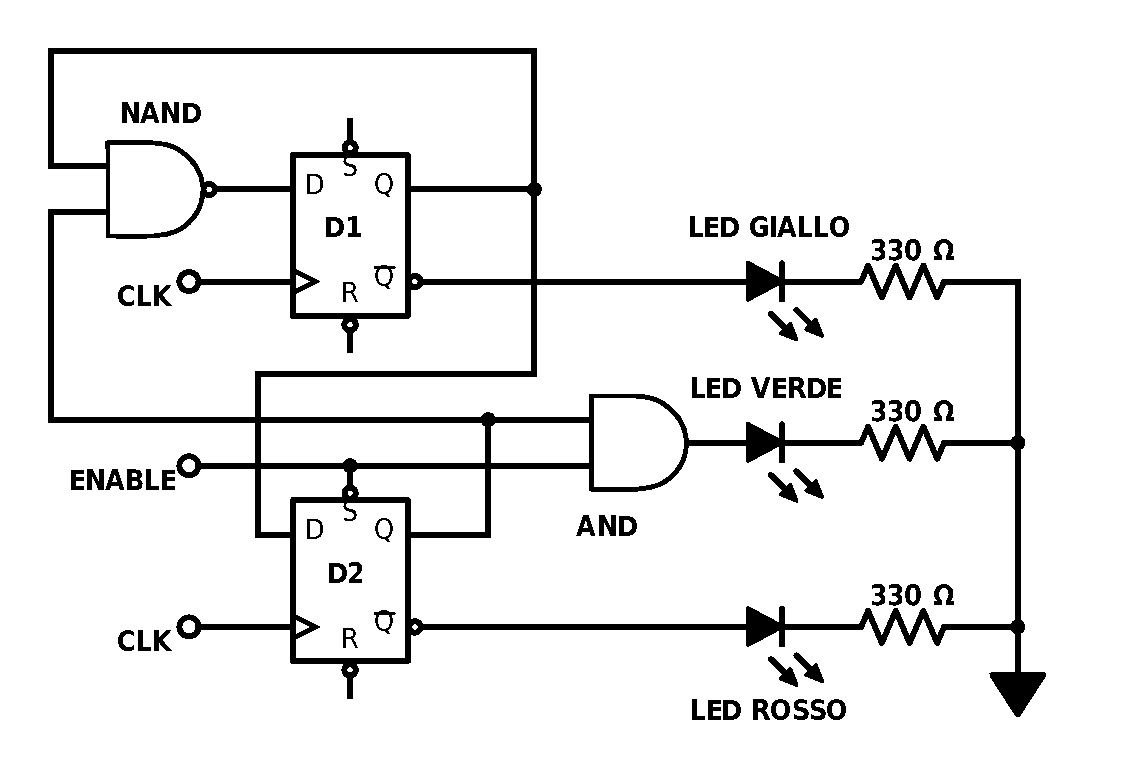
\includegraphics[scale=0.45]{with_enable.pdf}
	\caption{Circuito che realizzi il semaforo con segnale di Enable.}
	\label{fig:encirc}
\end{figure}

Come già notato, tale implementazione non è sincrona; nel caso si desiderasse renderla tale sarebbe necessario passare ad un'implementazione come macchina di Moore, ad esempio introducendo un ulteriore D-Latch che abbia in ingresso $En$:
dimostrativamente è stato realizzato il circuito in \fig{syncen}, verificandone il comportamento sincrono e il rispetto delle specifiche.

Passando ad una macchina di Moore non è possibile utilizzare meno di 3 flip-flop, dal momento che gli stati richiesti sono più di 4.

\begin{figure}[h]
	\centering
	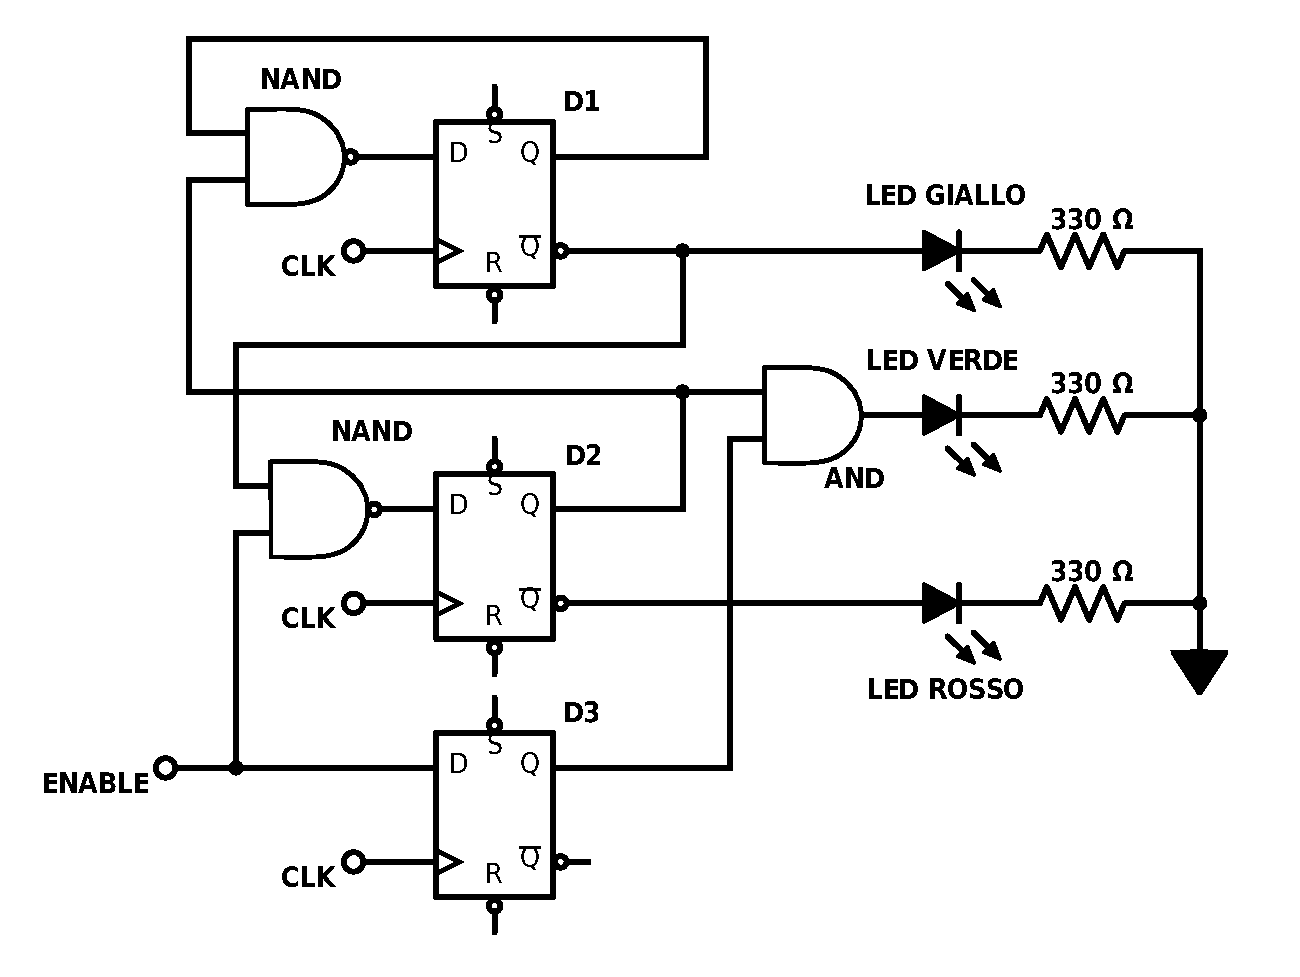
\includegraphics[scale=0.45]{sync_enable.pdf}
	\caption{Circuito che realizzi il semaforo con segnale di Enable in modo sincrono.}
	\label{fig:syncen}
\end{figure}
